\section*{One Game, Two Logics}
Consider a system that is described by the value of two different components:
Xolor (pronounced color) and Pattern. Each component has two values when
measured: red/blue for Xolor and solid/design for Pattern. A four-sided die
(tetrahedron) can represent each pair of component values on its faces for a
classical game (see following table).
\begin{tabular}{ccc}
  \toprule
  \multicolumn{1}{c}{\bfseries Xolor ($X$)} %
  &\multicolumn{2}{c}{\bfseries Pattern ($P$)} %
  \\%
  \cmidrule(lr){2-3}
  &\multicolumn{1}{c}{solid ($s$)} %
  &\multicolumn{1}{c}{design ($d$)} %
  \\%
  \midrule
  red ($r$)%
  &\raisebox{-0.5\height}{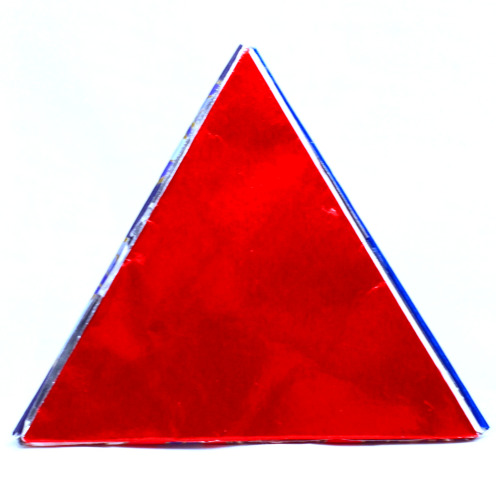
\includegraphics[scale=0.66]{Graphics/XrPs-scaled}} %
  &\raisebox{-0.5\height}{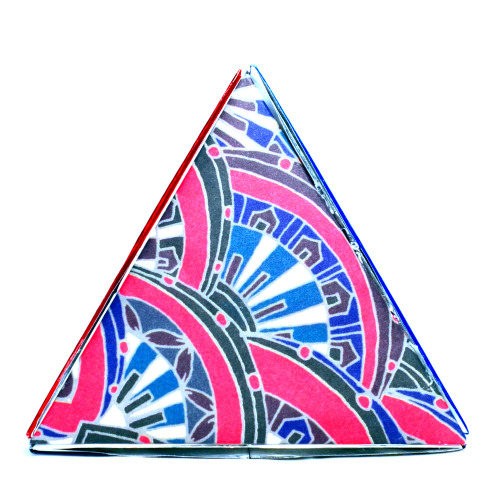
\includegraphics[scale=0.65]{Graphics/XrPd-scaled}} %
  \\%
  blue ($b$)%
  &\raisebox{-0.5\height}{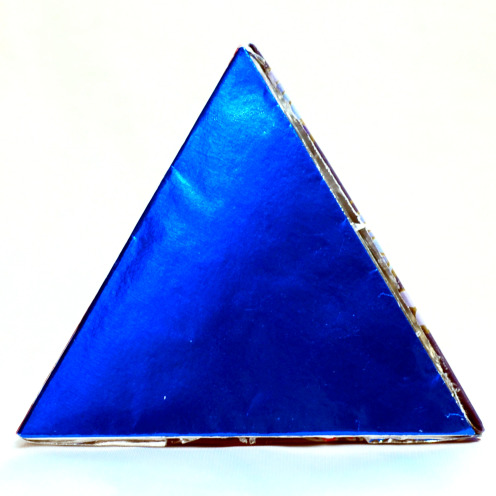
\includegraphics[scale=0.75, trim={0.15cm 0.15cm
        0.15cm 0.15cm}, clip]{Graphics/XbPs-scaled}} %
  &\raisebox{-0.5\height}{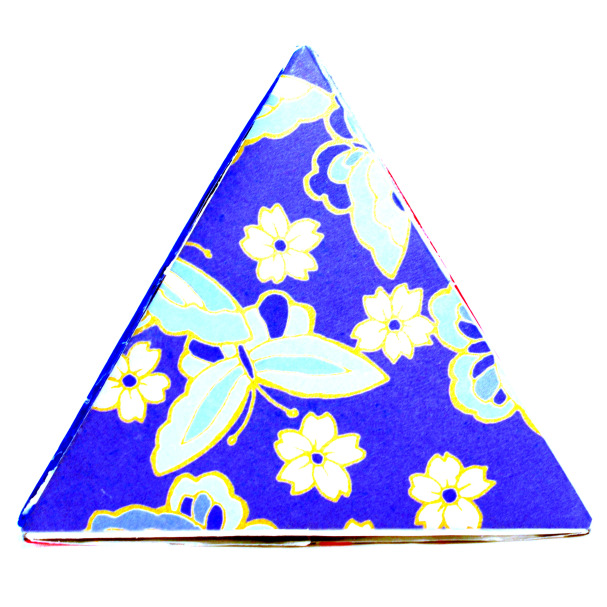
\includegraphics[scale=0.6]{Graphics/XbPd-scaled}}
  %
  \\%
  \bottomrule
\end{tabular}

There are two players, the Classical (C) and Quantum Scientist (Q). Both
are honest and both have a firm grasp of classical reasoning. The only
difference is that C does not know quantum mechanical reasoning whereas Q
does.  Game play for a single round proceeds in four stages: Setup,
Guess, Verify, and Score. 
\begin{enumerate}
\item Setup: Q \emph{prepares} the system and honestly records the results of
  \emph{measuring} the components in succession, $X$ then $P$. Note:
  Measuring with the tetrahedron described previously means observing the
  face of the die that is down, and \emph{only for that component being
    measured at the moment}; any other presumed information is not
  regarded. 
\item Guess: C guesses the state of the system by recording the values
  that $X$ and $P$ hold simultaneously at this stage of play.
\item Verify: Q \emph{measures} the components of the system again in
  succession, $X$ then $P$.
\item Score: Together C and Q compare the verified values to the guessed
  values. If the results of $X$ {\bfseries and} $P$ match then C gains
  \$1. If the results do not \emph{both} match then C losses \$2.
\end{enumerate}
The Scientists agree to play ten rounds, five with a classical system and
five with a quantum system. 

%\subsection*{The Classical System: Common Reasoning}
\begingroup
\setlength{\tabcolsep}{4 pt}
\begin{table}[H]
  \centering
  \caption{\emph{Classical} system play results (actual)}
\begin{tabular}{*{6}{>$l<$}}
  \toprule
  \multicolumn{2}{c}{\bfseries Setup}
  &\multicolumn{1}{c}{\bfseries Guess}
  &\multicolumn{2}{c}{\bfseries Verify}
  &\multicolumn{1}{c}{\bfseries Score}
  \\%
  \cmidrule(lr){1-2} %
  %\cmidrule(lr){3-3} %
  \cmidrule(lr){4-5} %
  %
  \multicolumn{1}{c}{$\Downarrow\!\! X$}
  &\multicolumn{1}{c}{$\Downarrow\!\! P$}
  &\multicolumn{1}{c}{$(X \text{ \bfseries and } P)$}
  &\multicolumn{1}{c}{$\Downarrow\!\! X$}
  &\multicolumn{1}{c}{$\Downarrow\!\! P$}
  %&\multicolumn{1}{c}{$\Downarrow\!\! X$}
  \\%
  \midrule
  b & d & (b,d) & b & d & +\$1\\%
  b & s & (b,s) & b & s & +\$1\\%
  b & s & (b,s) & b & s & +\$1\\%
  r & d & (r,d) & r & d & +\$1\\%
  r & s & (r,s) & r & s & +\$1\\%
  \bottomrule
\end{tabular}
\end{table}
\endgroup


\begingroup
\setlength{\tabcolsep}{4 pt}
\vspace*{-2\baselineskip}%
\begin{table}[H]
  \centering
  \caption{\emph{Quantum} system play results (actual)}
\begin{tabular}{*{6}{>$l<$}}
  \toprule
  \multicolumn{2}{c}{\bfseries Setup}
  &\multicolumn{1}{c}{\bfseries Guess}
  &\multicolumn{2}{c}{\bfseries Verify}
  &\multicolumn{1}{c}{\bfseries Score}
  \\%
  \cmidrule(lr){1-2} %
  %\cmidrule(lr){3-3} %
  \cmidrule(lr){4-5} %
  %
  \multicolumn{1}{c}{$\Downarrow\!\! X$}
  &\multicolumn{1}{c}{$\Downarrow\!\! P$}
  &\multicolumn{1}{c}{$(X \text{ \bfseries and } P)$}
  &\multicolumn{1}{c}{$\Downarrow\!\! X$}
  &\multicolumn{1}{c}{$\Downarrow\!\! P$}
  %&\multicolumn{1}{c}{$\Downarrow\!\! X$}
  \\%
  \midrule
  b & d & (b,d) & b & s & -\$2\\%
  b & d & (b,s) & r & s & -\$2\\%
  b & s & (b,s) & b & s & +\$1\\%
  r & s & (r,d) & b & s & -\$2\\%
  r & s & (r,s) & r & s & +\$1\\%
  \bottomrule
\end{tabular}
\end{table}
\endgroup

At the end of this particular game the C is up \$1, which seems good to C
especially since he has the classical half of the game down pat. Before
continuing with another game, the Classical Scientist would be wise to not
be beguiled and should consider the following, {\bfseries the Quantum house
  always wins!} Using classical reasoning with quantum systems is a losing
proposition\footnote{%
  Hint: {\bfseries Quantum measurement prepares the system} into a particular
  state. Component measurements are not necessarily simultaneously
  compatible, thereby randomizing the results of successive measurements. % 
}.

